\begin{figure}[tbp]\centering
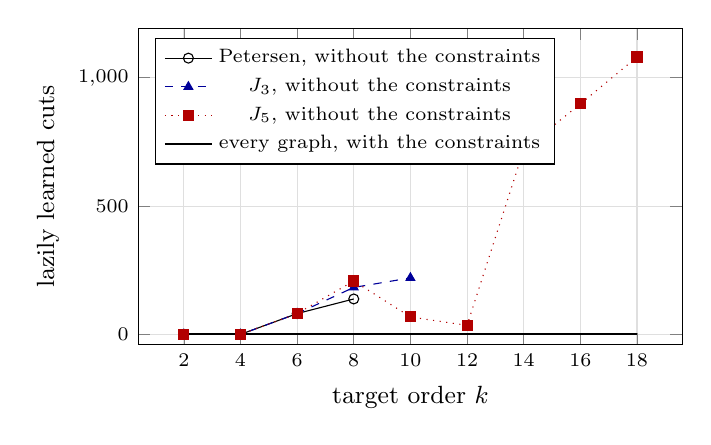
\begin{tikzpicture}
\pgfplotsset{every axis/.append style={tick label style={font=\scriptsize}, label style={font=\small}, legend style={font=\scriptsize}, grid=major, grid style={gray!25}}}
\begin{axis}[width=0.7\textwidth, height=5.6cm, xlabel={target order $k$}, ylabel={lazily learned cuts}, legend pos=north west, ymin=-40, xtick={2,4,6,8,10,12,14,16,18}]
\addplot[mark=o, mark options={solid}, mark size=1.8pt, thin, black, solid] coordinates {(2,0) (4,0) (6,81) (8,138)};
\addlegendentry{Petersen, without the constraints}
\addplot[mark=triangle*, mark options={solid}, mark size=1.8pt, thin, blue!60!black, dashed] coordinates {(2,0) (4,0) (6,81) (8,183) (10,220)};
\addlegendentry{$J_3$, without the constraints}
\addplot[mark=square*, mark options={solid}, mark size=1.8pt, thin, red!70!black, dotted] coordinates {(2,0) (4,0) (6,81) (8,208) (10,68) (12,35) (14,720) (16,898) (18,1081)};
\addlegendentry{$J_5$, without the constraints}
\addplot[thick, black, domain=2:18] {0};
\addlegendentry{every graph, with the constraints}
\end{axis}
\end{tikzpicture}
\caption{Lazily learned connectivity and bridge cuts on the control instances against the target order $k$: the formula without the fiber constraints (markers) and the formula with them (solid line at zero, all 21 instances). The number of cuts of the formula without the constraints grows with the order.}\label{fig:ablation}
\end{figure}
